% ============================================================
%  PrepMeUp - teknisk oplaeg
%  Beamer, 16:9. Kompilerer med pdfLaTeX.
%  Selvstaendig fil - ingen billeder eller eksterne filer.
% ============================================================
\documentclass[aspectratio=169,10pt]{beamer}

\usepackage[T1]{fontenc}
\usepackage[utf8]{inputenc}
\usepackage[danish]{babel}
\usepackage{lmodern}
\usepackage{booktabs}
\usepackage{array}
\usepackage{tikz}
\usetikzlibrary{positioning,arrows.meta,fit,backgrounds,calc}

% ---------- tema ----------
\usetheme{default}
\usecolortheme{default}
\setbeamertemplate{navigation symbols}{}

\definecolor{pine}{HTML}{264B44}
\definecolor{deep}{HTML}{173330}
\definecolor{moss}{HTML}{4E7A5F}
\definecolor{signal}{HTML}{C99700}
\definecolor{alert}{HTML}{9B3A2C}
\definecolor{soft}{HTML}{5A6B68}
\definecolor{faint}{HTML}{8B9A97}
\definecolor{rule}{HTML}{CCD4D1}
\definecolor{paper}{HTML}{F4F6F4}
\definecolor{mossbg}{HTML}{EEF3F0}
\definecolor{signalbg}{HTML}{FBF5E3}

\setbeamercolor{background canvas}{bg=paper}
\setbeamercolor{frametitle}{fg=deep}
\setbeamercolor{framesubtitle}{fg=soft}
\setbeamercolor{normal text}{fg=deep}
\setbeamercolor{structure}{fg=pine}
\setbeamerfont{frametitle}{size=\Large,series=\bfseries}
\setbeamerfont{framesubtitle}{size=\scriptsize,family=\ttfamily}

\setbeamertemplate{frametitle}{%
  \vspace{5mm}%
  \usebeamerfont{frametitle}\usebeamercolor[fg]{frametitle}\insertframetitle\par
  \ifx\insertframesubtitle\@empty\else
    \vspace{1mm}\usebeamerfont{framesubtitle}\usebeamercolor[fg]{framesubtitle}\insertframesubtitle\par
  \fi
  \vspace{1.5mm}%
}
\setbeamertemplate{footline}{%
  \hfill{\tiny\ttfamily\color{faint}\insertframenumber\,/\,\inserttotalframenumber}\hspace{6mm}\vspace{2.5mm}%
}

% ---------- hjaelpere ----------
\newcommand{\hd}[1]{{\ttfamily\bfseries\color{deep}#1}}
\newcommand{\bottomnote}[1]{\vfill{\scriptsize\color{soft}#1}\vspace{1.5mm}}
\newcommand{\punkt}[2]{%
  \item[\textcolor{signal}{\rule{1.2pt}{4mm}}]
  {\large\bfseries\color{deep}#1}\\[1mm]{\small\color{soft}#2}}

\tikzset{
  box/.style   ={draw=pine,  line width=.6pt, fill=white,    align=left, inner sep=5pt, text width=32mm, font=\tiny},
  boxc/.style  ={draw=moss,  line width=.6pt, fill=mossbg,   align=left, inner sep=5pt, text width=32mm, font=\tiny},
  boxd/.style  ={draw=signal,line width=.6pt, fill=signalbg, align=left, inner sep=5pt, text width=32mm, font=\tiny},
  boxx/.style  ={draw=faint, line width=.6pt, fill=paper,    align=left, inner sep=5pt, text width=32mm, font=\tiny},
  bnd/.style   ={draw=rule,  line width=.6pt, dashed, rounded corners=2pt, inner sep=4mm},
  ln/.style    ={draw=pine,  line width=.7pt, -{Latex[length=1.6mm]}},
  lns/.style   ={draw=signal,line width=1pt,  -{Latex[length=2mm]}},
  lnd/.style   ={draw=faint, line width=.6pt, dashed, -{Latex[length=1.6mm]}},
  life/.style  ={draw=rule,  line width=.5pt, dotted},
  tag/.style   ={font=\tiny\ttfamily, color=moss},
  bndlbl/.style={font=\tiny\ttfamily, color=faint},
}

% ============================================================
\begin{document}

% ---------- 1 forside ----------
{
\setbeamercolor{background canvas}{bg=pine}
\begin{frame}[plain]
  \vspace{12mm}
  {\color{white}\fontsize{40}{44}\selectfont\bfseries PrepMeUp}\\[6mm]
  {\color{paper}\large Teknisk oplæg: arkitektur, repo og udviklingsopsætning}\\[14mm]
  {\color{faint}\ttfamily\footnotesize Gruppe 3 \quad SW4PRJ4 \quad 4.\ semester softwareteknologi}
\end{frame}
}

% ---------- 2 stakken ----------
\begin{frame}{Stakken}{seks valg, resten følger af dem}
  \vspace{2mm}
  \renewcommand{\arraystretch}{1.5}
  \begin{tabular}{@{}p{34mm}p{34mm}p{34mm}@{}}
    \toprule
    {\ttfamily\scriptsize\color{signal} kunde-app} &
    {\ttfamily\scriptsize\color{signal} admin-ui} &
    {\ttfamily\scriptsize\color{signal} backend} \\
    \textbf{Expo} \newline {\scriptsize\color{soft} React Native, TypeScript, Expo Router} &
    \textbf{React} \newline {\scriptsize\color{soft} Vite, TypeScript} &
    \textbf{ASP.NET Core} \newline {\scriptsize\color{soft} Web API, .NET 10} \\[4mm]
    {\ttfamily\scriptsize\color{signal} data} &
    {\ttfamily\scriptsize\color{signal} test} &
    {\ttfamily\scriptsize\color{signal} udvikling} \\
    \textbf{SQL via EF Core} \newline {\scriptsize\color{soft} i Docker, ens på Windows og Linux} &
    \textbf{NUnit + Vitest} \newline {\scriptsize\color{soft} NSubstitute, GitHub Actions} &
    \textbf{Claude Code} \newline {\scriptsize\color{soft} 4 agenter, 11 skills, Kaneo} \\
    \bottomrule
  \end{tabular}
  \bottomnote{Én backend, to brugerflader, én delt klientpakke genereret fra OpenAPI.}
\end{frame}

% ---------- 3 containere ----------
\begin{frame}{Containere}{kørende processer og protokoller}
  \centering
  \resizebox{0.97\linewidth}{!}{%
  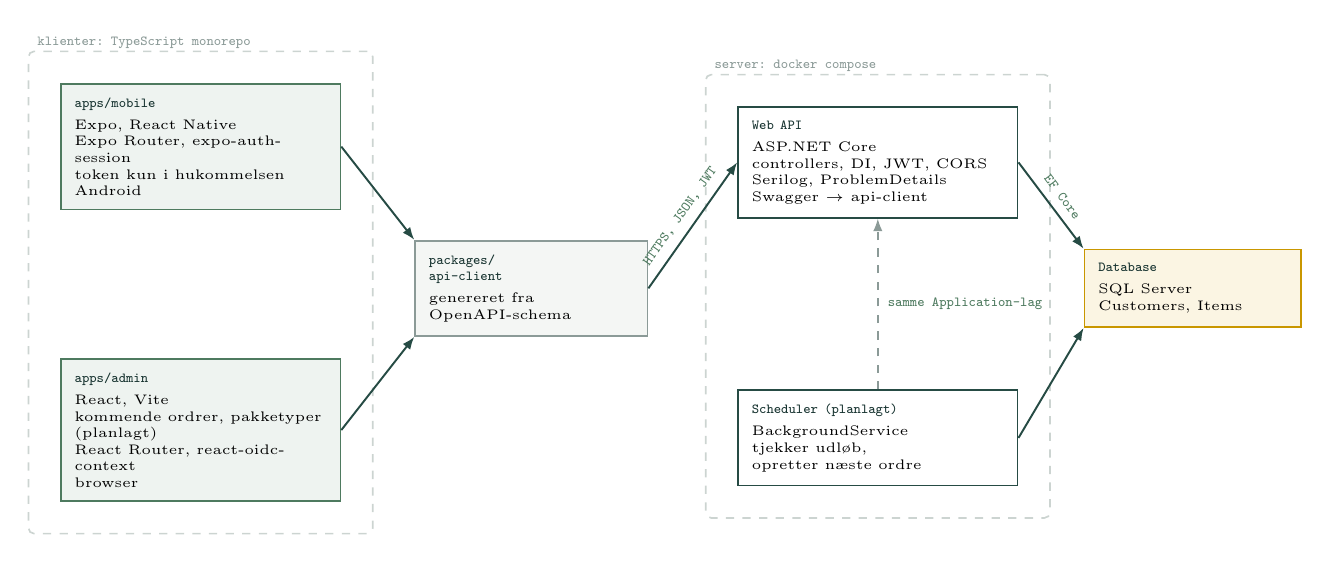
\begin{tikzpicture}
    \node[boxc] (mob) at (0,1.8)
      {\hd{apps/mobile}\\[2pt] Expo, React Native\\ Expo Router, expo-auth-session\\ token kun i hukommelsen\\ Android};
    \node[boxc] (adm) at (0,-1.8)
      {\hd{apps/admin}\\[2pt] React, Vite\\ kommende ordrer, pakketyper (planlagt)\\ React Router, react-oidc-context\\ browser};
    \node[boxx,text width=26mm] (cli) at (4.2,0)
      {\hd{packages/}\\ \hd{api-client}\\[2pt] genereret fra\\ OpenAPI-schema};
    \node[box] (api) at (8.6,1.6)
      {\hd{Web API}\\[2pt] ASP.NET Core\\ controllers, DI, JWT, CORS\\ Serilog, ProblemDetails\\ Swagger $\rightarrow$ api-client};
    \node[box] (sch) at (8.6,-1.9)
      {\hd{Scheduler (planlagt)}\\[2pt] BackgroundService\\ tjekker udløb,\\ opretter næste ordre};
    \node[boxd,text width=24mm] (db) at (12.6,0)
      {\hd{Database}\\[2pt] SQL Server\\ Customers, Items};

    \begin{scope}[on background layer]
      \node[bnd,fit=(mob)(adm)] (b1) {};
      \node[bnd,fit=(api)(sch)] (b2) {};
    \end{scope}
    \node[bndlbl,above=1mm of b1.north west,anchor=west] {klienter: TypeScript monorepo};
    \node[bndlbl,above=1mm of b2.north west,anchor=west] {server: docker compose};

    \draw[ln] (mob.east) -- (cli.north west);
    \draw[ln] (adm.east) -- (cli.south west);
    \draw[ln] (cli.east) -- node[tag,above,sloped] {HTTPS, JSON, JWT} (api.west);
    \draw[ln] (api.east) -- node[tag,above,sloped] {EF Core} (db.north west);
    \draw[ln] (sch.east) -- (db.south west);
    \draw[lnd] (sch.north) -- node[tag,right] {samme Application-lag} (api.south);
  \end{tikzpicture}}
  \bottomnote{Kontrakten mellem klient og server er OpenAPI-schemaet.}
\end{frame}

% ---------- 4 lag (koncept) ----------
\begin{frame}{Hvad er et lag?}{en gruppe klasser med ét fælles ansvar}
  \centering
  \resizebox{0.90\linewidth}{!}{%
  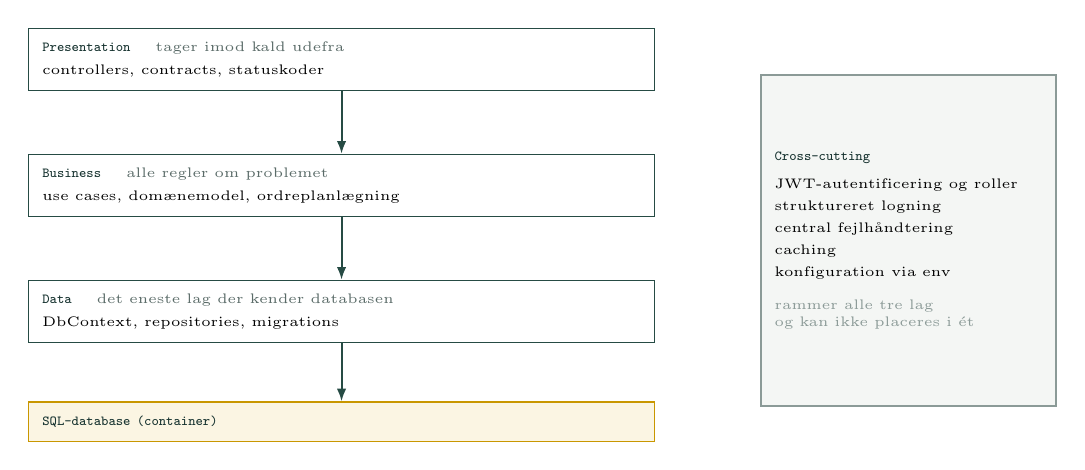
\begin{tikzpicture}
    \node[box,text width=76mm] (l1) at (0,3)
      {\hd{Presentation} \quad {\color{soft}tager imod kald udefra}\\[2pt] controllers, contracts, statuskoder};
    \node[box,text width=76mm] (l2) at (0,1.4)
      {\hd{Business} \quad {\color{soft}alle regler om problemet}\\[2pt] use cases, domænemodel, ordreplanlægning};
    \node[box,text width=76mm] (l3) at (0,-0.2)
      {\hd{Data} \quad {\color{soft}det eneste lag der kender databasen}\\[2pt] DbContext, repositories, migrations};
    \node[boxd,text width=76mm] (l4) at (0,-1.6)
      {\hd{SQL-database (container)}};
    \draw[ln] (l1) -- (l2);
    \draw[ln] (l2) -- (l3);
    \draw[ln] (l3) -- (l4);
    \node[boxx,text width=34mm,minimum height=42mm] (cc) at (7.2,0.7)
      {\hd{Cross-cutting}\\[4pt]
       JWT-autentificering og roller\\[2pt]
       struktureret logning\\[2pt]
       central fejlhåndtering\\[2pt]
       caching\\[2pt]
       konfiguration via env\\[6pt]
       {\color{faint} rammer alle tre lag\\ og kan ikke placeres i ét}};
  \end{tikzpicture}}
  \bottomnote{\textbf{Et lag må kun bruge laget under sig.} Derfor kan vi skifte database uden at røre reglerne, og teste reglerne uden en database.}
\end{frame}

% ---------- 5 lagreglerne ----------
\begin{frame}{Lagreglerne}{står også i AGENTS.md, så agenterne arbejder efter dem}
  \vspace{1mm}
  \scriptsize
  \renewcommand{\arraystretch}{1.35}
  \begin{tabular}{@{}>{\ttfamily\color{deep}}p{22mm}p{52mm}p{45mm}@{}}
    \toprule
    \normalfont\color{soft}\ttfamily modul & \color{soft}\ttfamily må & \color{soft}\ttfamily må ikke \\
    \midrule
    Api & route, validere, mappe contract mod domæne, statuskoder, autorisation & forretningsregler; kende {\ttfamily DbContext} \\
    Application & orkestrere use cases, definere repository-interfaces, transaktionsgrænser & kende HTTP, {\ttfamily ControllerBase}, EF-typer, SQL \\
    Domain & entiteter, invarianter, vandbehov, pakkeindhold, udløb & referere til noget andet projekt overhovedet \\
    Infrastructure & EF-konfiguration, queries, migrations & træffe beslutninger. Den henter og gemmer \\
    clients/apps & kalde API'et via {\ttfamily api-client}, holde UI-state & duplikere forretningsregler; gå uden om klientpakken \\
    \bottomrule
  \end{tabular}
  \bottomnote{Lagene bliver til fire projekter i solution. Næste slide viser hvem der må referere hvem.}
\end{frame}

% ---------- 6 modulafhaengigheder ----------
\begin{frame}{Modulafhængigheder}{de samme fire lag, nu som projekter. Pilen peger mod det, der refereres}
  \centering
  \resizebox{0.88\linewidth}{!}{%
  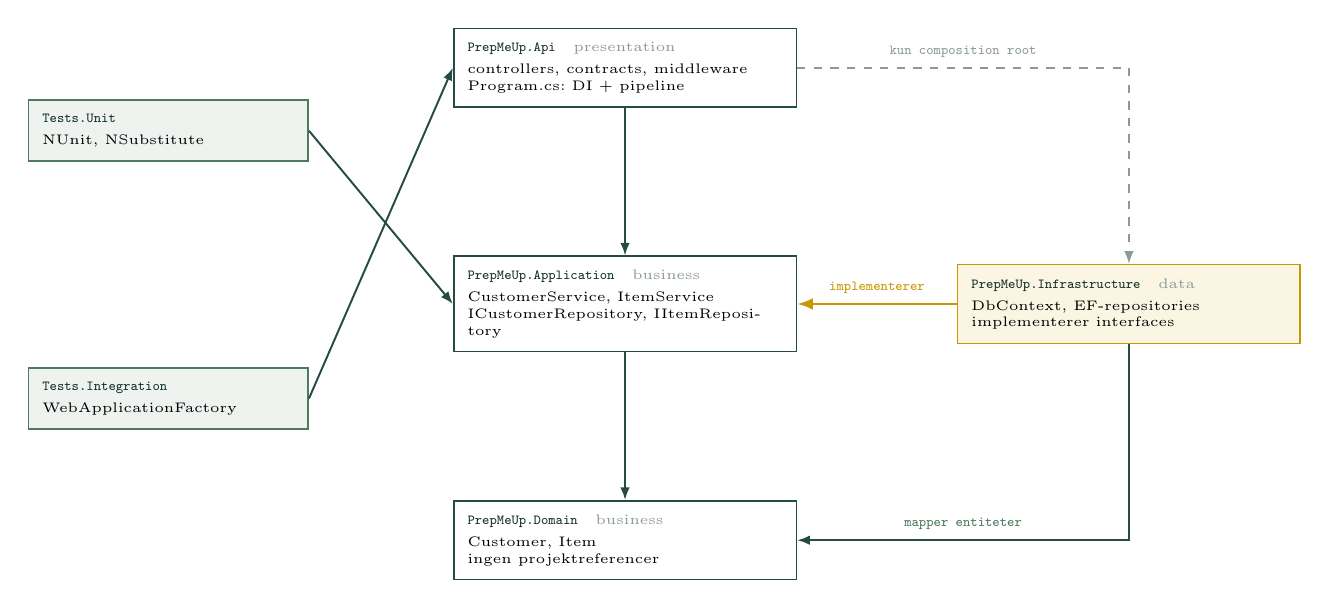
\begin{tikzpicture}
    \node[box,text width=40mm] (apip) at (4,3)
      {\hd{PrepMeUp.Api} \; {\color{faint}presentation}\\[2pt] controllers, contracts, middleware\\ Program.cs: DI + pipeline};
    \node[box,text width=40mm] (app) at (4,0)
      {\hd{PrepMeUp.Application} \; {\color{faint}business}\\[2pt] CustomerService, ItemService\\ ICustomerRepository, IItemRepository};
    \node[box,text width=40mm] (dom) at (4,-3)
      {\hd{PrepMeUp.Domain} \; {\color{faint}business}\\[2pt] Customer, Item\\ ingen projektreferencer};
    \node[boxd,text width=40mm] (inf) at (10.4,0)
      {\hd{PrepMeUp.Infrastructure} \; {\color{faint}data}\\[2pt] DbContext, EF-repositories\\ implementerer interfaces};
    \node[boxc,text width=32mm] (tu) at (-1.8,2.2)
      {\hd{Tests.Unit}\\[2pt] NUnit, NSubstitute};
    \node[boxc,text width=32mm] (ti) at (-1.8,-1.2)
      {\hd{Tests.Integration}\\[2pt] WebApplicationFactory};

    \draw[ln] (apip) -- (app);
    \draw[ln] (app)  -- (dom);
    \draw[lns] (inf.west) -- node[tag,above,color=signal] {implementerer} (app.east);
    \draw[ln] (inf.south) |- node[tag,above,pos=.75] {mapper entiteter} (dom.east);
    \draw[lnd] (apip.east) -| node[bndlbl,above,pos=.25] {kun composition root} (inf.north);
    \draw[ln] (tu.east) -- (app.west);
    \draw[ln] (ti.east) -- (apip.west);
  \end{tikzpicture}}
  \bottomnote{\textbf{Domain refererer ingenting.} Derfor kan forretningsreglerne testes uden database, browser eller HTTP. Den gule pil vender ind mod domænet i stedet for ud mod databasen.}
\end{frame}

% ---------- 7 EF Core = SQL ----------
\begin{frame}[fragile]{EF Core kort fortalt}{I har haft SQL. EF Core skriver SQL'en for jer.}
  \vspace{1mm}
  {\scriptsize\color{soft} En \emph{object-relational mapper}: C\#-klasser bliver til tabeller, og LINQ bliver til SQL. Vi kan altid se den genererede SQL og skrive den i hånden, hvor det er nødvendigt.}
  \vspace{3mm}

  \begin{columns}[T,onlytextwidth]
    \begin{column}{0.47\textwidth}
      {\tiny\ttfamily\color{moss} vi skriver dette i C\#}\\[1mm]
      \begin{semiverbatim}
\tiny\ttfamily
var customer = await db.Customers
    .SingleOrDefaultAsync(
        c => c.KeycloakId == keycloakId);
      \end{semiverbatim}
    \end{column}
    \begin{column}{0.5\textwidth}
      {\tiny\ttfamily\color{moss} EF Core sender dette til databasen}\\[1mm]
      \begin{semiverbatim}
\tiny\ttfamily
SELECT TOP(2) c.*
FROM Customers AS c
WHERE c.KeycloakId = @keycloakId
      \end{semiverbatim}
    \end{column}
  \end{columns}

  \vspace{2mm}
  \tiny
  \renewcommand{\arraystretch}{1.2}
  \begin{tabular}{@{}>{\ttfamily\color{deep}}p{38mm}p{42mm}p{45mm}@{}}
    \toprule
    \normalfont\color{soft}\ttfamily i C\# & \color{soft}\ttfamily i SQL & \color{soft}\ttfamily bemærk \\
    \midrule
    class Customer         & {\ttfamily CREATE TABLE Customers} & én klasse, én tabel \\
    List$<$Order$>$ Orders & fremmednøgle + {\ttfamily JOIN}    & kaldes en navigation (Order er planlagt) \\
    SaveChangesAsync()     & {\ttfamily INSERT}/{\ttfamily UPDATE} i én transaktion & alt eller intet \\
    migration              & versionsstyrede {\ttfamily ALTER TABLE}-scripts & ligger i git \\
    \bottomrule
  \end{tabular}
\end{frame}

% ---------- 8 sekvens ----------
\begin{frame}{Ét kald gennem stakken}{PUT /user}
  \centering
  \resizebox{0.95\linewidth}{!}{%
  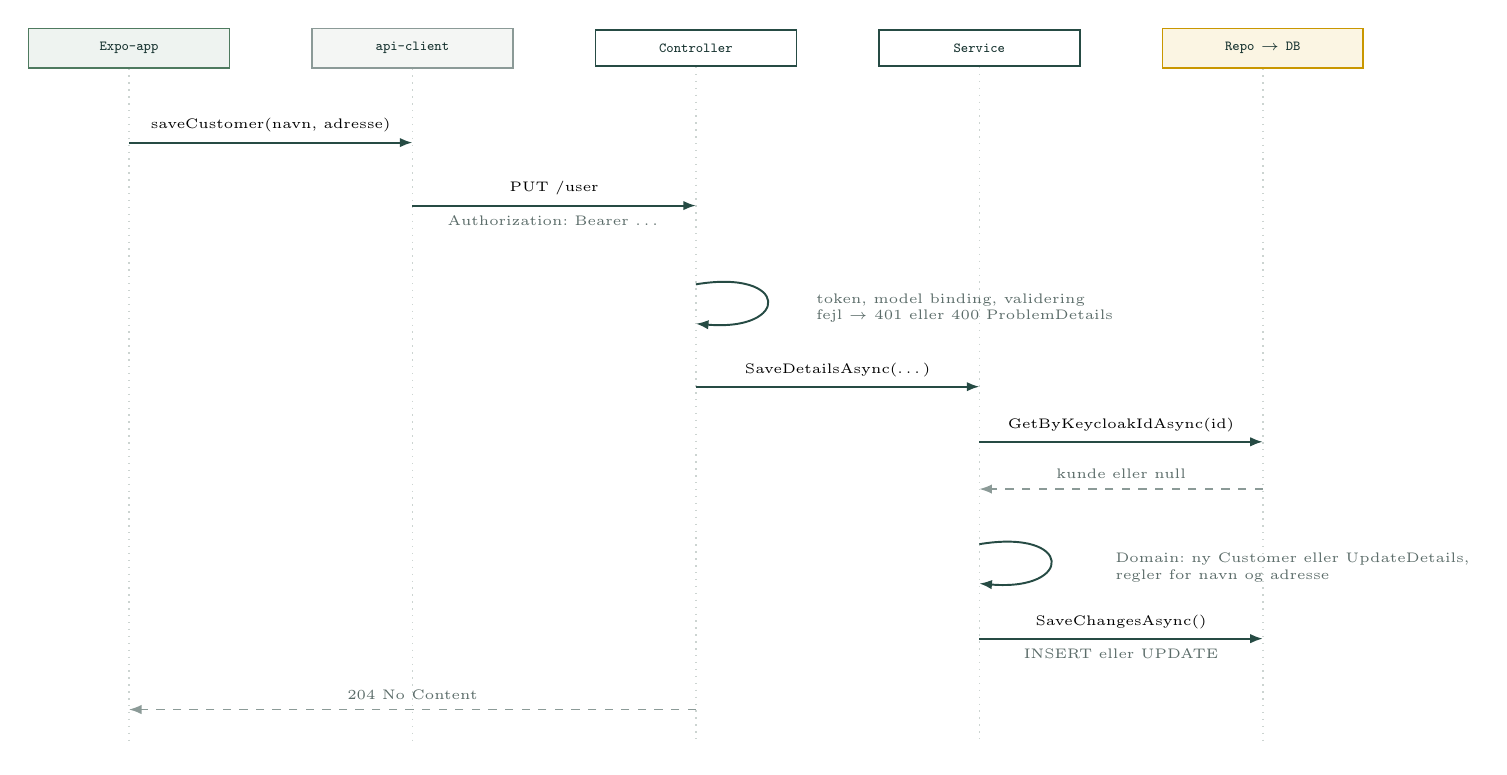
\begin{tikzpicture}[font=\tiny]
    \def\yT{0} \def\yB{-8.6}
    \node[boxc,text width=22mm,align=center] (c1) at (0,\yT)  {\hd{Expo-app}};
    \node[boxx,text width=22mm,align=center] (c2) at (3.6,\yT) {\hd{api-client}};
    \node[box, text width=22mm,align=center] (c3) at (7.2,\yT) {\hd{Controller}};
    \node[box, text width=22mm,align=center] (c4) at (10.8,\yT){\hd{Service}};
    \node[boxd,text width=22mm,align=center] (c5) at (14.4,\yT){\hd{Repo $\rightarrow$ DB}};

    \foreach \n in {c1,c2,c3,c4,c5} \draw[life] (\n.south) -- ($(\n.south)+(0,\yB)$);

    \draw[ln] (0,-1.2) -- node[above]{saveCustomer(navn, adresse)} (3.6,-1.2);
    \draw[ln] (3.6,-2.0) -- node[above]{PUT /user} node[below,color=soft]{Authorization: Bearer \ldots} (7.2,-2.0);
    \draw[ln] (7.2,-3.0) .. controls (8.4,-2.8) and (8.4,-3.6) .. (7.2,-3.5)
          node[right,xshift=14mm,yshift=2mm,color=soft,align=left]{token, model binding, validering\\ fejl $\rightarrow$ 401 eller 400 ProblemDetails};
    \draw[ln] (7.2,-4.3) -- node[above]{SaveDetailsAsync(\ldots)} (10.8,-4.3);
    \draw[ln] (10.8,-5.0) -- node[above]{GetByKeycloakIdAsync(id)} (14.4,-5.0);
    \draw[lnd] (14.4,-5.6) -- node[above,color=soft]{kunde eller null} (10.8,-5.6);
    \draw[ln] (10.8,-6.3) .. controls (12.0,-6.1) and (12.0,-6.9) .. (10.8,-6.8)
          node[right,xshift=16mm,yshift=2mm,color=soft,align=left]{Domain: ny Customer eller UpdateDetails,\\ regler for navn og adresse};
    \draw[ln] (10.8,-7.5) -- node[above]{SaveChangesAsync()} node[below,color=soft]{INSERT eller UPDATE} (14.4,-7.5);
    \draw[lnd] (7.2,-8.4) -- node[above,color=soft]{204 No Content} (0,-8.4);
  \end{tikzpicture}}
  \bottomnote{Læg mærke til, at kaldet går præcis én vej ned gennem lagene og samme vej tilbage.}
\end{frame}

% ---------- 9 deployment ----------
\begin{frame}{Deployment}{udviklingsopsætning}
  \centering
  \resizebox{0.82\linewidth}{!}{%
  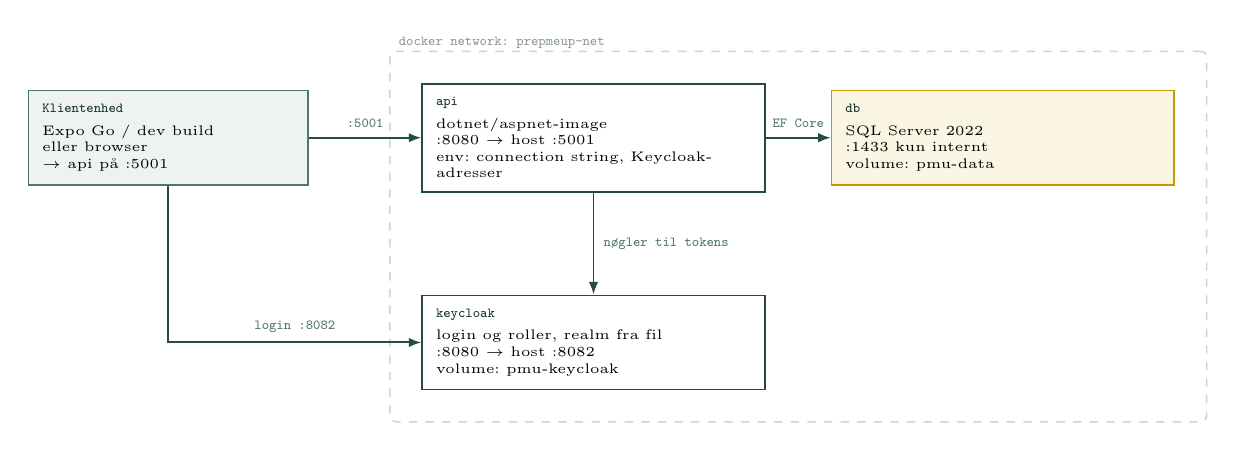
\begin{tikzpicture}
    \node[boxc,text width=32mm] (cl) at (0,0)
      {\hd{Klientenhed}\\[2pt] Expo Go / dev build\\ eller browser\\ $\rightarrow$ api på :5001};
    \node[box,text width=40mm] (api) at (5.4,0)
      {\hd{api}\\[2pt] dotnet/aspnet-image\\ :8080 $\rightarrow$ host :5001\\ env: connection string, Keycloak-adresser};
    \node[boxd,text width=40mm] (db) at (10.6,0)
      {\hd{db}\\[2pt] SQL Server 2022\\ :1433 kun internt\\ volume: pmu-data};
    \node[box,text width=40mm] (kc) at (5.4,-2.6)
      {\hd{keycloak}\\[2pt] login og roller, realm fra fil\\ :8080 $\rightarrow$ host :8082\\ volume: pmu-keycloak};
    \begin{scope}[on background layer]
      \node[bnd,fit=(api)(db)(kc)] (net) {};
    \end{scope}
    \node[bndlbl,above=1mm of net.north west,anchor=west] {docker network: prepmeup-net};
    \draw[ln] (cl) -- node[tag,above]{:5001} (api);
    \draw[ln] (cl.south) |- node[tag,above,pos=.75]{login :8082} (kc.west);
    \draw[ln] (api) -- node[tag,above]{EF Core} (db);
    \draw[ln] (api) -- node[tag,right]{nøgler til tokens} (kc);
  \end{tikzpicture}}
  \bottomnote{Databasen eksponeres ikke til host. Kun api-containeren når den, via servicenavnet db. Derfor er opsætningen ens på Windows og Linux. Logning skrives med Serilog til konsollen.}
\end{frame}

% ---------- 10 repoet ----------
\begin{frame}[fragile]{Repoet}{mapperne under src/ svarer 1:1 til modulerne}
  \vspace{1mm}
\begin{semiverbatim}
\tiny\ttfamily
prepmeup/
|-- AGENTS.md                     \color{faint}# lagregler, konventioner, definition of done\color{deep}
|-- CLAUDE.md                     \color{faint}# peger paa AGENTS.md + det Claude-specifikke\color{deep}
|-- .claude/
|   |-- settings.json             \color{faint}# naegter adgang til .env og noeglefiler\color{deep}
|   |-- agents/                   \color{faint}# 4 read-only reviewere\color{deep}
|   `-- skills/                   \color{faint}# 11 arbejdsgange\color{deep}
|-- src/
|   |-- PrepMeUp.Domain/          \color{moss}// ingen referencer\color{deep}
|   |-- PrepMeUp.Application/     \color{moss}// interfaces + use cases\color{deep}
|   |-- PrepMeUp.Infrastructure/  \color{moss}// EF Core\color{deep}
|   `-- PrepMeUp.Api/             \color{moss}// HTTP (BackgroundService planlagt)\color{deep}
|-- clients/
|   |-- AGENTS.md                 \color{faint}# TS strict, ingen forretningslogik i UI\color{deep}
|   |-- apps/mobile/              \color{faint}# Expo\color{deep}
|   |-- apps/admin/               \color{faint}# React + Vite\color{deep}
|   `-- packages/api-client/      \color{faint}# genereret - redigeres ikke i haanden\color{deep}
|-- tests/
|   |-- PrepMeUp.Tests.Unit/
|   `-- PrepMeUp.Tests.Integration/
|-- docs/                         \color{faint}# rapport og bilag i LaTeX\color{deep}
|-- docker-compose.yml
`-- .github/workflows/            \color{faint}# CI og tjek af konventioner\color{deep}
\end{semiverbatim}
\end{frame}

% ---------- 11 udviklingsopsaetning ----------
\begin{frame}{Udviklingsopsætning}{værktøj omkring repoet, som ikke kører i produktion}
  \centering
  \resizebox{0.95\linewidth}{!}{%
  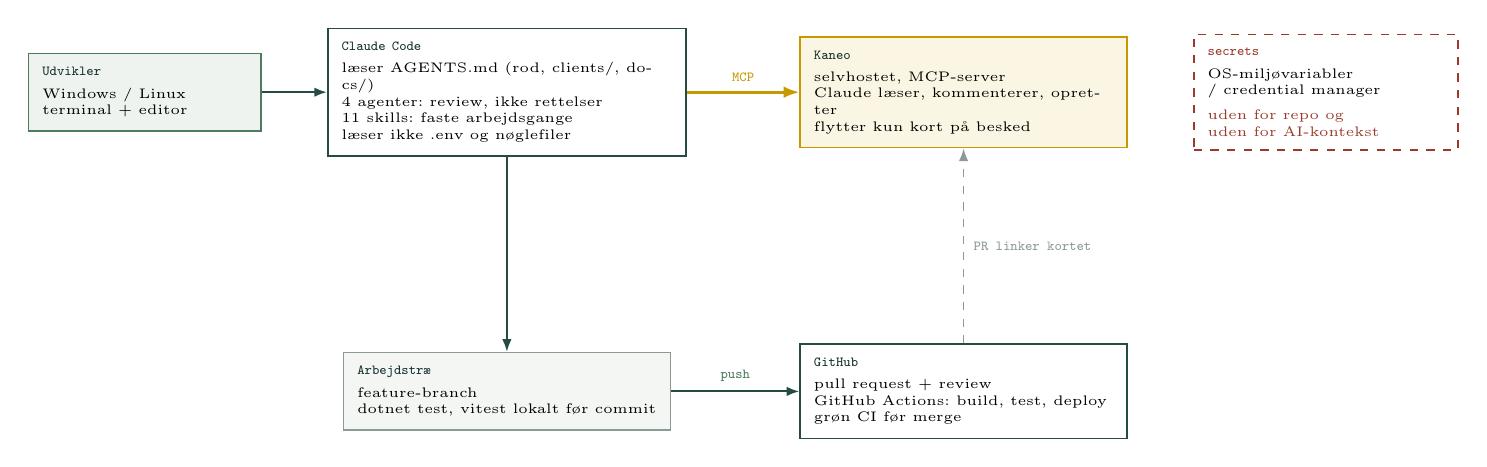
\begin{tikzpicture}
    \node[boxc,text width=26mm] (dev) at (0,1.4)
      {\hd{Udvikler}\\[2pt] Windows / Linux\\ terminal + editor};
    \node[box,text width=42mm] (cc) at (4.6,1.4)
      {\hd{Claude Code}\\[2pt] læser AGENTS.md (rod, clients/, docs/)\\ 4 agenter: review, ikke rettelser\\ 11 skills: faste arbejdsgange\\ læser ikke .env og nøglefiler};
    \node[boxx,text width=38mm] (wt) at (4.6,-2.4)
      {\hd{Arbejdstræ}\\[2pt] feature-branch\\ dotnet test, vitest lokalt før commit};
    \node[box,text width=38mm] (gl) at (10.4,-2.4)
      {\hd{GitHub}\\[2pt] pull request + review\\ GitHub Actions: build, test, deploy\\ grøn CI før merge};
    \node[boxd,text width=38mm] (kn) at (10.4,1.4)
      {\hd{Kaneo}\\[2pt] selvhostet, MCP-server\\ Claude læser, kommenterer, opretter\\ flytter kun kort på besked};
    \node[draw=alert,dashed,line width=.6pt,text width=30mm,align=left,inner sep=5pt,font=\tiny] (sec) at (15.0,1.4)
      {{\ttfamily\bfseries\color{alert}secrets}\\[2pt] OS-miljøvariabler\\ / credential manager\\[3pt] {\color{alert}uden for repo og\\ uden for AI-kontekst}};

    \draw[ln] (dev) -- (cc);
    \draw[ln] (cc.south) -- (wt.north);
    \draw[ln] (wt) -- node[tag,above]{push} (gl);
    \draw[lns] (cc.east) -- node[tag,above,color=signal]{MCP} (kn.west);
    \draw[lnd] (gl.north) -- node[bndlbl,right]{PR linker kortet} (kn.south);
  \end{tikzpicture}}
  \bottomnote{Kaneo-login sker med device-login i browseren, så der ligger intet Kaneo-token i miljøet eller i en fil. Secrets til databasen og Keycloak kommer fra miljøet og aldrig fra en fil, agenten kan læse.}
\end{frame}

% ---------- 12 agenterne ----------
\begin{frame}{Agenterne}{fire reviewere, alle read-only}
  \vspace{1mm}
  \tiny
  \renewcommand{\arraystretch}{1.4}
  \begin{tabular}{@{}>{\ttfamily\color{deep}}p{30mm}p{60mm}p{34mm}@{}}
    \toprule
    \normalfont\color{soft}\ttfamily agent & \color{soft}\ttfamily rolle & \color{soft}\ttfamily kaldes \\
    \midrule
    architecture-reviewer & lagregler, afhængighedsretning, SOLID, design smells & før hver pull request \\
    backend-reviewer      & REST, statuskoder, model binding, EF-model, N+1, migrations & ved nye endpoints og før merge \\
    test-designer         & ækvivalensklasser, grænseværdier, fakes, integrationsplan & før tests skrives \\
    security-reviewer     & auth (Keycloak, JWT), adgangskontrol, secrets, validering & før deployment \\
    \bottomrule
  \end{tabular}
\end{frame}

% ---------- 13 skills ----------
\begin{frame}{Skills}{elleve faste arbejdsgange}
  \vspace{1mm}
  \scriptsize
  \renewcommand{\arraystretch}{1.0}
  \begin{tabular}{@{}>{\ttfamily\color{deep}}p{32mm}p{95mm}@{}}
    \toprule
    \normalfont\color{soft}\ttfamily skill & \color{soft}\ttfamily hvad den gør \\
    \midrule
    vertical-slice   & ny funktion gennem alle lag i rigtig rækkefølge, Domain først og skærmen til sidst \\
    tdd-loop         & red-green-refactor med NUnit og NSubstitute, testtilfældene godkendes først \\
    api-contract     & holder OpenAPI-dokumentet og api-client i sync (NSwag) \\
    git-workflow     & branch fra main, commit, pull request mod main, release-tag \\
    plan             & ny plan i .plans/ med en interaktiv HTML-side \\
    report-check     & kritik af rapporten og optælling mod 72.000 tegn \\
    student-voice    & omskriver et bilag til almindelig studenterstemme \\
    meeting-docs     & dagsordener og referater på dansk i LaTeX \\
    drawio-skill     & draw.io-diagrammer til rapport og bilag \\
    oral-examiner    & eksaminerer jer i jeres eget projekt \\
    defend-my-code   & forbereder dig på at forklare dine egne commits \\
    \bottomrule
  \end{tabular}
\end{frame}

% ---------- 14 graenser ----------
\begin{frame}{Grænserne vi har sat}{tre bevidste begrænsninger på hvad agenten må}
  \vspace{1mm}
  \begin{itemize}\setlength\itemsep{4mm}
    \punkt{Agenterne retter ikke koden}{De rapporterer fund med fil, linje og forslag. Når du selv retter fundet, kan du forklare det til eksamen.}
    \punkt{Testdesign er delt i to}{Agenten test-designer foreslår testtilfældene og begrunder dem. Først når et menneske har godkendt listen, implementerer skillen tdd-loop dem. Testdesign er et læringsmål i softwaretest.}
    \punkt{Claude flytter kun kort på besked}{Claude læser, kommenterer og opretter kort. Når et gruppemedlem beder om det, flytter og estimerer Claude dem, men tildeler eller sletter aldrig. Hvilke kort der flyttes, er gruppens beslutning. Den iterative proces er et læringsmål, og tavlens historik bliver procesbilag i rapporten.}
  \end{itemize}
  \bottomnote{Samme princip gælder report-check, oral-examiner og defend-my-code: de stiller spørgsmål og kritiserer, men skriver ikke rapportprosaen.}
\end{frame}

% ---------- 15 ordforklaring ----------
\begin{frame}{Tre ord der er faldet undervejs}{}
  \vspace{3mm}
  \begin{itemize}\setlength\itemsep{5mm}
    \punkt{Vertical slice}{Vi bygger én funktion hele vejen igennem, fra skærm til database, frem for ét lag ad gangen. Hver iteration ender med noget, der virker, i stedet for tre færdige lag og ingen funktion.}
    \punkt{Clean Architecture}{Et udbredt navn for den lagdeling, vi bruger, hvor afhængighederne peger ind mod domænet. Kurset kalder det \emph{Layers}, og det er det ord, vi bruger i rapporten.}
    \punkt{MediatR}{Et bibliotek, der lægger et mellemled ind mellem controller og logik. \textbf{Vi bruger det ikke}, fordi det løser et problem, vi ikke har endnu, og det står ikke i pensum.}
  \end{itemize}
\end{frame}

\end{document}
